\begin{frame}
  \frametitle{strace}
  System call tracer\\
  \url{https://sourceforge.net/projects/strace/}
  \begin{itemize}
  \item Available on all GNU/Linux systems\\
    Can be built by your cross-compiling toolchain generator.
  \item Even easier: drop a ready-made static binary for your
        architecture, just when you need it. See
        \url{https://github.com/bootlin/static-binaries/tree/master/strace}
  \item Allows to see what any of your processes is doing:\\
    accessing files, allocating memory...\\
    Often sufficient to find simple bugs.
  \item Usage:\\
    \code{strace <command>} (starting a new process)\\
    \code{strace -p <pid>} (tracing an existing process)
    \code{strace -c <command>} (statistics of system calls taking most time)
  \end{itemize}
  See \code{man strace} for details.
\end{frame}

\begin{frame}[fragile]
  \frametitle{strace example output}
  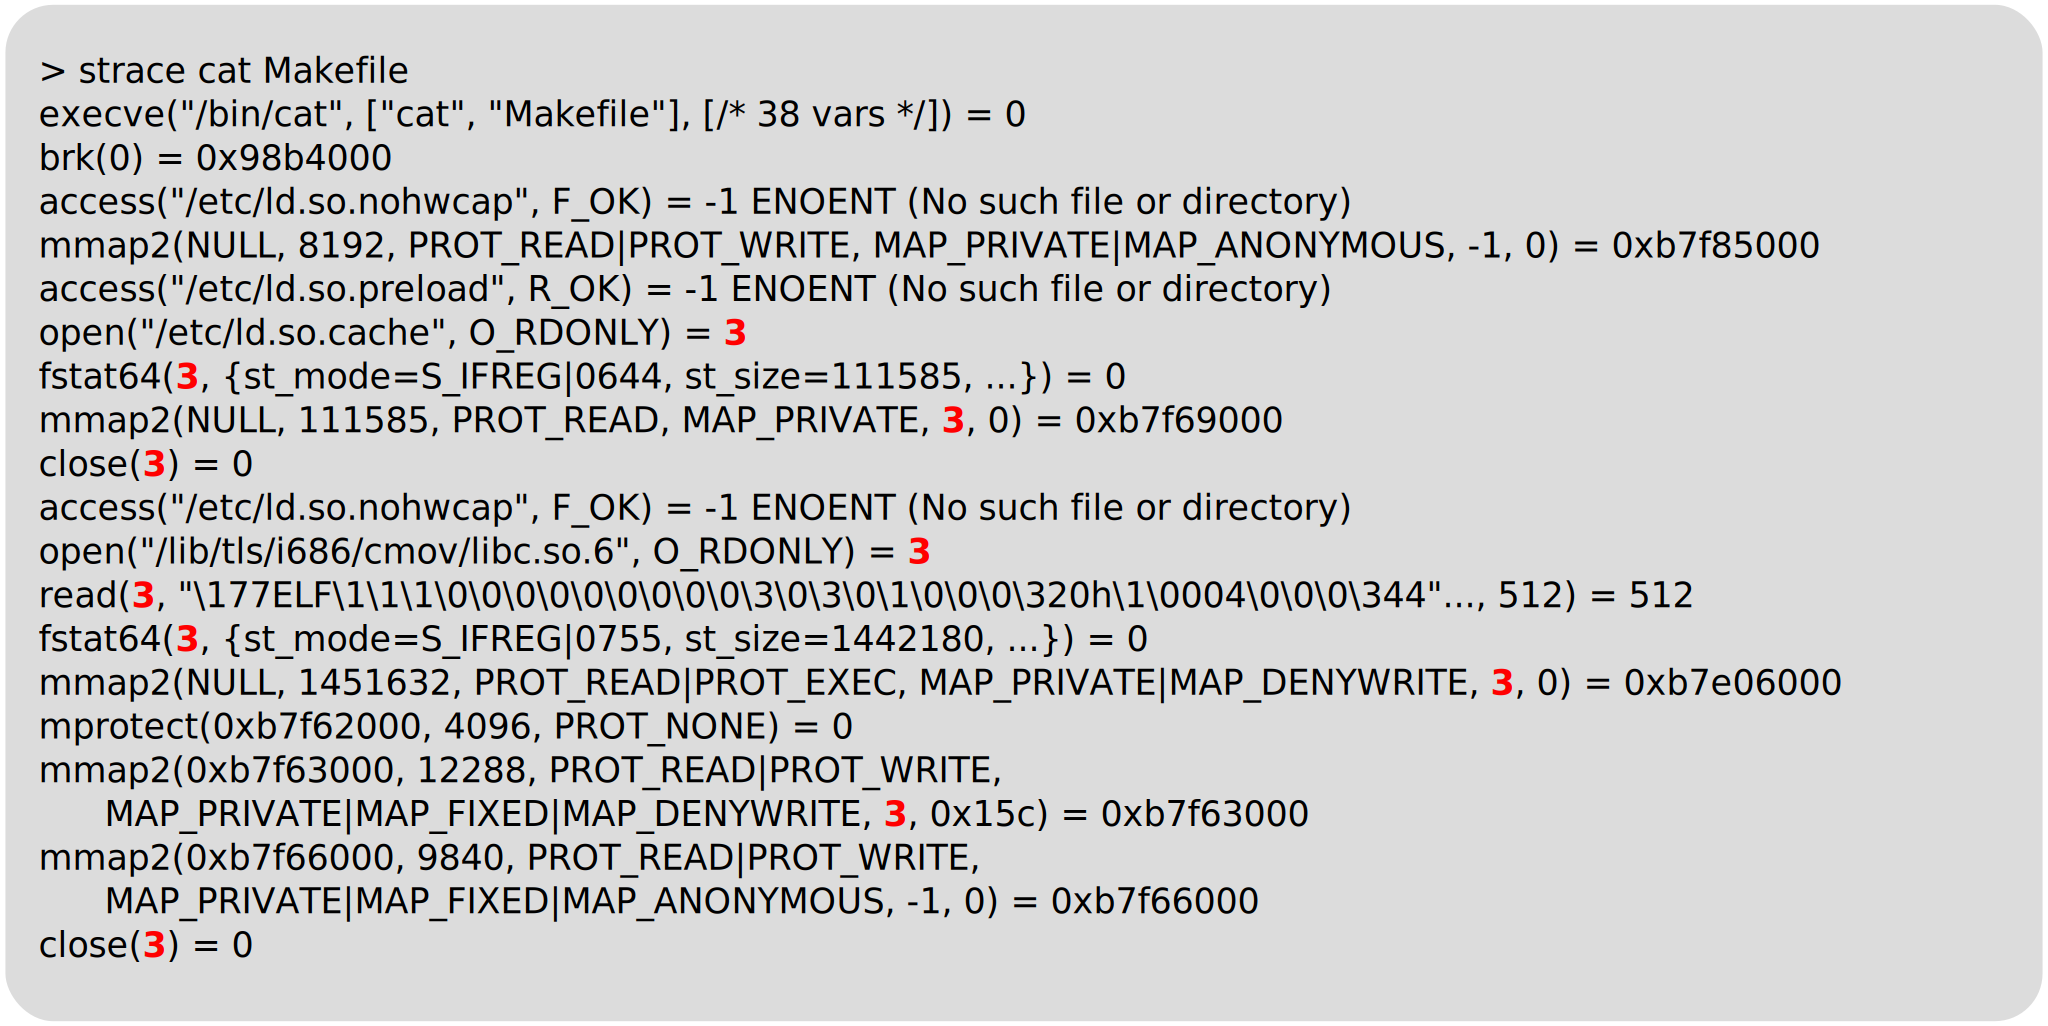
\includegraphics[width=\textwidth]{common/strace-output.pdf}\\
  Hint: follow the open file descriptors returned by \code{open()}. \\
  This tells you what files system calls are run on.
\end{frame}

\begin{frame}[fragile]
  \frametitle{strace -c example output}
  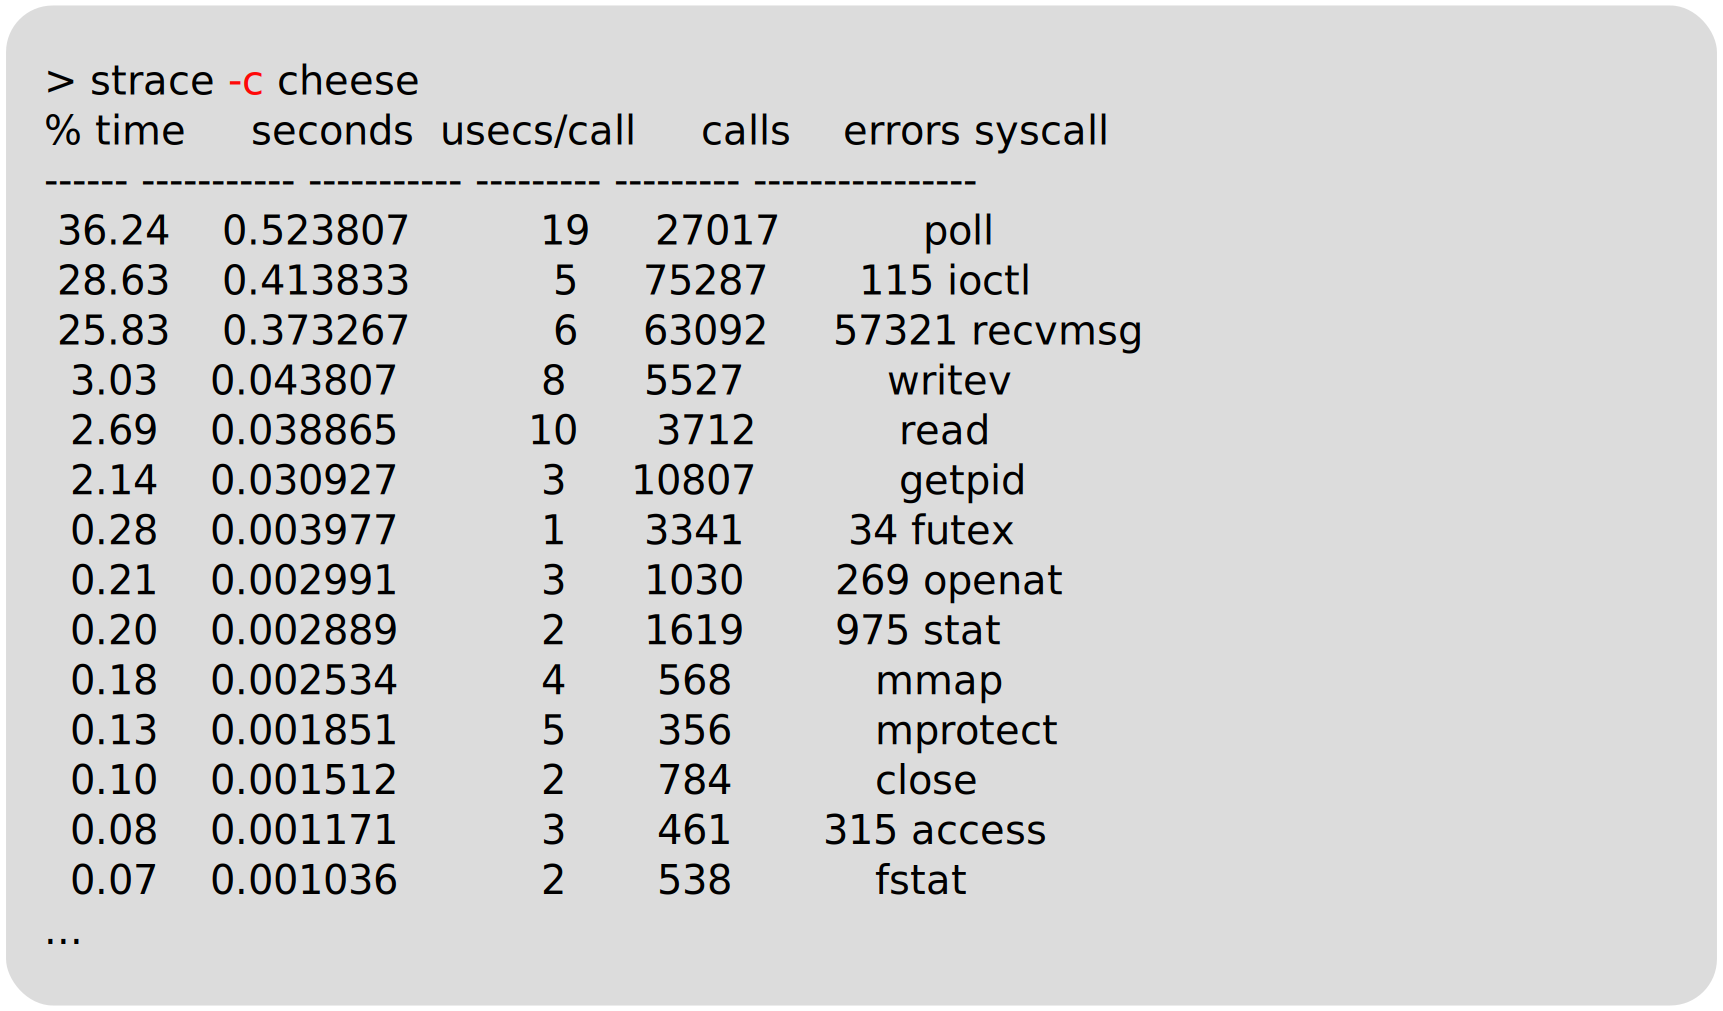
\includegraphics[height=0.8\textheight]{common/strace-c-output.pdf}
\end{frame}
